This chapter presents the conceptual foundation of the proposed solution, grounded in the requirements and limitations identified in Chapter 2. The core objective is to transform unstructured narrative input—whether spoken or typed—into structured, schema-conformant templates through a modular, agent-based architecture. Unlike monolithic approaches that attempt end-to-end extraction in a single inference step, the proposed system decomposes the task into specialized subtasks, each handled by a dedicated agent with clearly defined responsibilities and interfaces.

The design is motivated by three critical shortcomings observed in existing work. First, single-model systems lack transparency: when extraction fails, it is difficult to trace whether the error originated in entity recognition, field mapping, or format normalization \cite{du2021template, sun2023slot}. Second, monolithic architectures are brittle under noisy or domain-specific input, as they cannot isolate and recover from localized failures \cite{wang2021spoken}. Third, current solutions provide limited support for iterative refinement, user correction, or learning from domain knowledge, restricting their adaptability in real-world deployments \cite{mialon2023augmented, park2023generative}.

The proposed Invox system addresses these limitations through a five-stage pipeline that enforces separation of concerns while preserving end-to-end coherence. Each agent operates on well-defined inputs and produces structured outputs that serve as inputs to downstream components. This modular design directly supports the six requirements established in Section 2.1: consistency is enforced through dedicated normalization (R1), extraction accuracy benefits from retrieval-augmented context (R2), intermediate artifacts enable traceability (R3), outputs remain editable at the end before final submission (R4), the system learns from historical templates and domain resources (R5), and architectural strategies can be selected to meet latency constraints (R6).

The remainder of this chapter is organized as follows. Section 3.1 derives the conceptual design from the analysis results, explaining how each requirement motivates specific architectural decisions. Section 3.2 describes the five modular agents that comprise the pipeline, detailing their individual responsibilities, inputs, outputs, and internal mechanisms. Section 3.3 presents four architectural strategies—Single-Pass Full Input, Iterative Single-Field Processing, Multi-LLM Consensus (Full), and Multi-LLM Consensus (Iterative)—that instantiate the same pipeline with different trade-offs in accuracy, latency, and cost. Section 3.4 provides the high-level system architecture and design, including context diagrams, container views, and process flows that illustrate how components interact in deployment scenarios. Detailed implementation and experimental validation are deferred to Chapters 4 and 5, respectively.

% \section{Concept Derivation from Analysis Results}
\label{sec:concept-derivation}

The conceptual design of the Invox system is derived systematically from the six requirements identified in Section~\ref{sec:requirements} and the gaps observed in existing approaches reviewed in Section~\ref{sec:related-work}. This section traces how each architectural decision directly addresses specific limitations in current template-filling systems, establishing the rationale for a modular, multi-agent design.

\subsection{From Monolithic to Modular Processing}
\label{subsec:monolithic-to-modular}

The analysis in Section~\ref{sec:related-work} revealed that monolithic approaches—where a single LLM performs extraction, normalization, and validation in one inference step—suffer from three fundamental weaknesses. First, they propagate errors across stages without providing mechanisms for localized recovery \cite{sun2023slot}. When entity recognition fails, subsequent field mapping inherits these errors, compounding inaccuracies. Second, they lack transparency: users cannot trace which part of the input led to which output, making error diagnosis difficult and undermining trust \cite{ribeiro2016should}. Third, they provide no intermediate points for user intervention, forcing corrections to be applied post-hoc rather than during processing \cite{amershi2019guidelines}.

These observations directly motivate the decomposition of the template-filling task into discrete, sequential stages. By separating transcription, retrieval, extraction, normalization, and verification into dedicated agents, the system gains three critical capabilities. Errors can be isolated to specific stages, allowing targeted debugging and recovery without reprocessing the entire pipeline. Intermediate outputs become visible and editable, supporting both transparency (R3) and user correction (R4). Finally, individual agents can be improved or replaced independently, enabling iterative refinement without destabilizing the overall architecture.

\subsection{Addressing Consistency Through Dedicated Normalization}
\label{subsec:consistency-normalization}

Requirement R1 demands that heterogeneous inputs—whether informal speech transcripts, chat messages, or multilingual notes—be transformed into uniform, comparable template entries. Existing generative systems often produce stylistically inconsistent outputs because the same model is responsible for both content extraction and format enforcement \cite{huang2024authorship}. This dual responsibility introduces variance: one inference may produce "08/16/2025" while another outputs "August 16, 2025" for the same date, even when guided by identical prompts.

The solution is to delegate normalization to a specialized Consistency Formatting (CF) agent that operates independently of extraction. Once the Information Extraction (IE) agent proposes candidate values, CF applies deterministic transformations—date standardization, entity canonicalization, and vocabulary alignment—ensuring that all outputs conform to predefined schemas. This separation ensures that extraction logic remains focused on identifying correct content, while formatting logic enforces structural and stylistic uniformity. The result is higher consistency across diverse inputs, directly satisfying R1.

\subsection{Retrieval-Augmented Generation for Domain Adaptation}
\label{subsec:rag-domain-adaptation}

Requirement R2 emphasizes robust information extraction under noisy, incomplete, and domain-specific conditions. Section~\ref{sec:related-work} showed that zero-shot LLMs struggle with specialized terminology, abbreviations, and implicit references common in industrial and healthcare contexts \cite{wang2021spoken}. While few-shot prompting improves performance, manually curating examples for every deployment scenario is impractical and does not scale across domains \cite{wei2022emergent}.

This motivates the introduction of a Retrieval-Augmented Generation (RAG) agent positioned between transcription and extraction. The RAG agent queries an indexed corpus of historical templates and domain glossaries, retrieving the $k$ most semantically similar examples for the current input. These examples are passed to the IE agent as dynamic few-shot context, grounding its reasoning in domain-specific patterns without requiring manual prompt engineering. This design directly supports R2 by improving extraction accuracy on specialized vocabulary, and also contributes to R5 (learning and adaptation) by leveraging organizational knowledge accumulated over time.

\subsection{Verification for Completeness and Cross-Field Consistency}
\label{subsec:verification-consistency}

Existing template-filling systems rarely validate their own outputs. Once fields are populated, the result is presented to the user without checking for missing required fields, contradictory values, or schema violations \cite{sun2023slot}. This places the entire verification burden on the user, increasing workload and reducing trust.

The Verification (VER) agent addresses this gap by performing three types of checks after normalization. Completeness checks ensure that all required fields have been populated or explicitly marked as unavailable. Cross-field consistency checks detect contradictions, such as an incident date that falls outside the reported shift time. Confidence scoring highlights uncertain extractions, directing user attention to fields most likely to require correction. When issues are detected, VER can trigger a clarification loop, prompting the user for additional input before re-applying CF and VER on the updated values. This design supports R3 (transparency) by making verification criteria explicit, and R4 (user correction) by enabling targeted intervention.

\subsection{Modularity as a Foundation for Flexibility}
\label{subsec:modularity-flexibility}

The evaluation in Section~\ref{subsec:limitations} demonstrated that no single existing system satisfies all six requirements simultaneously. Systems optimized for accuracy often sacrifice latency \cite{park2023generative}, while those prioritizing speed compromise on transparency or adaptability \cite{google2024langextract}. This trade-off is inherent to monolithic designs, where architectural choices are baked into a single model and cannot be adjusted post-deployment.

The modular pipeline enables flexible deployment strategies without changing the underlying components. The same five agents can be orchestrated in multiple ways: as a sequential single-pass system for low-latency scenarios, as an iterative slot-parallel architecture for higher accuracy, or as a multi-model consensus mechanism for critical applications where reliability outweighs cost. Section~\ref{sec:architectural-strategies} formalizes these strategies and analyzes their trade-offs. This flexibility directly addresses R6 (usability) by allowing latency constraints to guide strategy selection, while preserving modularity for future improvements.


This section summarizes how each architectural decision maps to the requirements established in Chapter~\ref{chap:analysis}. The modular design is not an arbitrary choice, but a direct consequence of the limitations observed in existing work and the operational constraints of real-world deployment contexts. The next section details the five agents that instantiate this design, specifying their inputs, outputs, and internal processing logic.
% \section{Five-Agent Architecture}
\label{sec:concept-architecture}

The modular architecture of \textit{Invox} is organized into five specialized agents. Each agent exposes a clear input/output contract, enabling component-level analysis, flexible substitution, and isolated improvement. This section characterizes the roles of the agents and their interconnections, independent of any particular deployment strategy.

\begin{figure}[H]
  \centering
  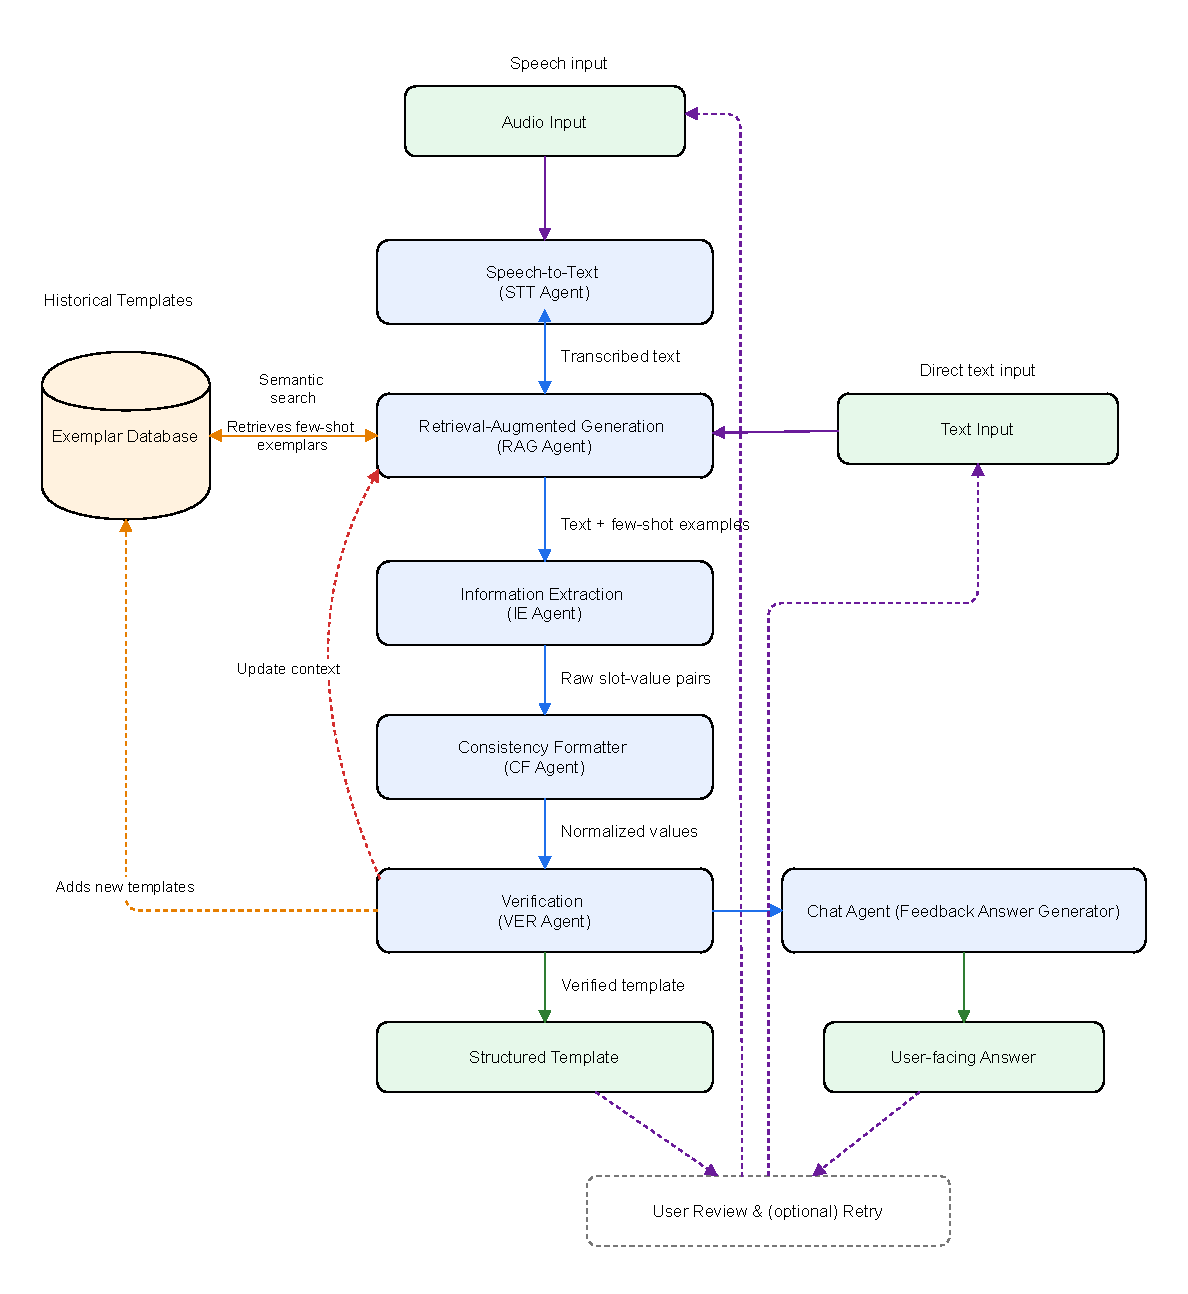
\includegraphics[width=1.0\linewidth]{images/agent_pipeline.drawio.pdf}
  \caption{Invox’s Five-Agent Pipeline}
  \label{fig:agent-pipeline}
\end{figure}



\subsection{Speech-to-Text Agent (STT)}
\label{subsec:stt-agent}

The STT agent converts spoken language into text using a Whisper-based transcription model \cite{radford2023whisper}. It accepts audio recordings as input and outputs transcribed text along with metadata such as word-level confidence scores, timestamps, and language detection results. As the focus of this work is the mapping from unstructured text to template fields, the STT component remains an adapter rather than the core of the architecture. Textual inputs bypass this stage and enter directly into the RAG agent.

\textbf{Design considerations.} The STT agent is deliberately shallow to maintain generality. Whisper was selected for its robustness to noise and multilingual support, which are critical in industrial environments where background machinery, accents, and code-switching are common \cite{fathullah2023prompting}. Alternative ASR systems could be substituted without affecting downstream components, provided they produce UTF-8 text output.

\subsection{Retrieval-Augmented Generation Agent (RAG)}
\label{subsec:rag-agent}

The RAG agent enhances extraction accuracy by retrieving relevant examples from historical data before template filling begins. It accepts the transcribed or typed text as input and queries an indexed corpus—comprising previously completed templates—using semantic similarity search over dense vector embeddings. The agent outputs the top-$k$ most relevant examples, which are passed alongside the user input to the IE agent as few-shot context.

\textbf{Retrieval mechanism.} The RAG agent encodes input text using a pretrained sentence transformer and performs cosine similarity search against stored template embeddings. The system returns $k$ ranked examples (typically $k = 3$–$5$), each containing the original text and its corresponding template completion.

\textbf{Design rationale.} This agent directly addresses R2 (information extraction) and R5 (learning and adaptation). By dynamically selecting examples tailored to the current input, the system avoids the brittleness of static few-shot prompts while benefiting from organizational memory \cite{mialon2023augmented}. The semantic search ensures that examples are retrieved based on conceptual similarity, making the system robust to paraphrasing and vocabulary variations. Over time, as more templates are completed and added to the index, extraction accuracy improves without requiring model retraining.

\subsection{Information Extraction Agent (IE)}
\label{subsec:ie-agent}

The IE agent performs the central task of transforming unstructured text into structured template fields. Its input consists of three components: (1) the free-form text (transcribed or provided directly), (2) the retrieved few-shot examples from the RAG agent, and (3) the target template schema specifying which fields need to be filled. The agent outputs candidate slot-value pairs for all specified fields in the template schema.

The agent operates by prompting a large language model with task-specific instructions and examples. For each field in the template schema, the model attempts to extract relevant information from the input text. If information for a particular field cannot be found in the text, the field is explicitly populated with a null value rather than being omitted. This ensures completeness while maintaining the structured output format.

\textbf{Processing approach:}
\begin{itemize}
    \item \textbf{Schema-driven extraction:} The agent processes all fields specified in the template schema, ensuring comprehensive coverage of the required information structure.
    \item \textbf{Evidence-based population:} Fields are populated only when supporting evidence is present in the input text, preventing hallucination of unsupported values.
    \item \textbf{Explicit null handling:} When information for a field is unavailable in the text, the field is explicitly marked as null, maintaining the complete output structure.
\end{itemize}

\textbf{Prompt structure.} The IE agent's prompt consists of four components: (1) task definition specifying the target schema and fields, (2) retrieved few-shot examples demonstrating successful extraction patterns, (3) the current user input text, and (4) output format constraints requiring JSON-structured responses that include all specified fields. This structure ensures consistent output formatting while leveraging the contextual understanding provided by few-shot examples \cite{zhang2023sgptod}.

\subsection{Consistency Formatting Agent (CF)}
\label{subsec:cf-agent}

The CF agent transforms the raw extracted values from the IE agent into standardized, schema-compliant formats. It accepts the slot-value pairs produced by the IE agent and applies deterministic normalization rules and schema validation to ensure consistency across all template outputs.

\textbf{Schema validation and normalization:}
\begin{itemize}
    \item \textbf{Data type enforcement:} Converts extracted values to appropriate data types (dates to ISO format, numbers to numerical types, etc.) and validates against schema constraints
    \item \textbf{Value canonicalization:} Standardizes variations using deterministic rules (e.g., ``Sept. 11'' → ``2001-09-11'', ``USA'' → ``United States'')
    \item \textbf{Controlled vocabulary mapping:} Enforces domain-specific conventions by mapping extracted terms to predefined categories for incident types, equipment codes, and other standardized fields
    \item \textbf{Schema compliance checking:} Validates that all values conform to the template schema requirements, including format constraints and value ranges
\end{itemize}

\textbf{Normalization approach.} The CF agent employs both deterministic transformations and LLM-based resolution for ambiguous cases. Structured data types like dates, numbers, and standard identifiers are normalized using regular expressions and parsing libraries. For ambiguous entities—such as informal location names or context-dependent equipment codes—the agent can prompt an LLM with the original context and domain glossaries to resolve variations. This hybrid approach balances precision with contextual awareness while maintaining deterministic behavior for well-defined formats.

\textbf{Design rationale.} By separating normalization from extraction, the system ensures consistent output formatting regardless of input variations while enforcing schema compliance. This addresses requirement R1 (consistency) and allows the IE agent to focus solely on content identification rather than format enforcement \cite{gatt2018survey}. The CF agent also reduces evaluation noise by ensuring that performance comparisons across different extraction strategies are not confounded by formatting inconsistencies.

\subsection{Verification Agent (VER)}
\label{subsec:ver-agent}

The VER agent performs comprehensive quality assessment on the structured template produced by the CF agent. It accepts the normalized slot-value pairs as input and generates a fully verified template with confidence scoring, field-level annotations, and interactive clarification capabilities.

\textbf{Quality assessment components:}
\begin{itemize}
    \item \textbf{Confidence scoring:} Assigns confidence scores to each populated field based on extraction quality, evidence strength, and internal consistency metrics
    \item \textbf{Field annotations:} Provides detailed annotations for each field indicating the source evidence, extraction method, and any processing notes
    \item \textbf{Conflict detection:} Identifies internal contradictions or inconsistencies between related fields (e.g., conflicting dates, incompatible equipment types)
    \item \textbf{Completeness validation:} Flags required fields that remain empty or contain insufficient information
\end{itemize}

\textbf{Interactive clarification system.} When low-confidence fields, conflicts, or missing required information are detected, the VER agent generates targeted chat messages to solicit user clarification. These messages are context-aware and focus specifically on the uncertain aspects of the template, enabling iterative refinement through user feedback. The system maintains conversation history to provide context for subsequent clarification rounds.

\textbf{Final output generation.} The VER agent produces the completed template with all quality annotations, making transparent which fields are highly reliable versus those requiring user verification. This includes:
\begin{itemize}
    \item Confidence scores for automated quality assessment
    \item Evidence references linking extracted values to source text spans
    \item Clear indicators of fields that may need user attention
    \item Structured data ready for database integration or further processing
\end{itemize}

\textbf{Design rationale.} VER directly supports R3 (transparency) by providing comprehensive field-level annotations and confidence metrics, and R4 (user correction) through its interactive clarification system. By centralizing quality assessment and user interaction in a dedicated agent, the system ensures consistent verification standards while maintaining clear separation from the extraction and normalization processes \cite{park2023generative}.

\subsection{Agent Interfaces and Data Flow}
\label{subsec:agent-interfaces}

Table~\ref{tab:agent-interfaces} summarizes the interface of each agent. By separating their responsibilities and outputs, the architecture supports substitution of different models, logging of intermediate states, and detailed error analysis. Figure~\ref{fig:agent-pipeline-enhanced} illustrates the sequential data flow through the five agents for both audio and text inputs.

\begin{table}[h]
\centering
\begin{tabular}{p{2.5cm}p{5cm}p{5.5cm}}
\toprule
\textbf{Agent} & \textbf{Input} & \textbf{Output} \\
\midrule
\textbf{STT} & Audio signal & Transcribed text with metadata (confidence scores, timestamps) \\
\midrule
\textbf{RAG} & Text (transcribed or direct input) & Top-$k$ retrieved examples with relevance scores and template mappings \\
\midrule
\textbf{IE} & Text + retrieved examples + template schema & Candidate slot-value pairs (null for unavailable fields) \\
\midrule
\textbf{CF} & Raw slot-value pairs & Normalized values with schema validation and format standardization \\
\midrule
\textbf{VER} & Normalized slot-value pairs & Verified template with confidence scores, field annotations, and clarification prompts \\
\bottomrule
\end{tabular}
\caption{Invox's Agent interfaces and data flow}
\label{tab:agent-interfaces}
\end{table}

The next section formalizes four deployment strategies that instantiate this architecture with different orchestration patterns, trading off accuracy, latency, and computational cost.


% \section{Architectural Strategies}
\label{sec:architectural-strategies}

While the modular five-agent pipeline defines the general structure of the \textit{Invox} system, its effectiveness depends on how large language models (LLMs) are deployed within the \textit{Information Extraction} and \textit{Verification} stages. Different architectural strategies offer distinct trade-offs in terms of accuracy, robustness, latency, cost, and transparency. This section outlines four strategies and illustrates them using a common example to enable direct comparison.

For all examples, we use the following input derived from the MUC-4 benchmark:  
\textit{``On March 3, 1992, in Bogotá, a powerful car bomb exploded outside the Ministry of Defense, damaging nearby buildings and injuring 25 people, though no fatalities were reported. Authorities suspect a left-wing guerrilla group, but responsibility remains unconfirmed.''}

This example introduces multiple attributes (date, location, event type, casualties, suspected perpetrators, and epistemic uncertainty), allowing us to highlight the strengths and weaknesses of each strategy under realistic conditions.

\subsection{Strategy S1: Single-Pass (Full-Input, Single-LLM)}
\label{subsec:strategy-s1}

\textbf{Overview.}  
In the simplest approach, a single LLM receives the complete transcript—along with few-shot examples retrieved by the RAG agent—and directly generates all template fields in one inference pass. The extracted values then proceed through Consistency Formatting (CF) and Verification (VER) before finalization.

\begin{figure}[H]
  \centering
  \includegraphics[width=1.0\linewidth]{images/single-llm-full-input.drawio.pdf}
  \caption{Strategy: Full-Input, Single-LLM}
  \label{fig:single-llm-full-input}
\end{figure}

\textbf{Advantages.}  
This strategy is computationally efficient, requiring only one IE model call. It minimizes latency and API costs, making it suitable for high-throughput scenarios. The inclusion of RAG-retrieved examples improves domain adaptation compared to zero-shot prompting, while CF and VER stages provide downstream quality assurance.

\textbf{Limitations.}  
If the LLM misinterprets a critical ambiguity—such as treating ``suspected guerrilla group'' as a confirmed perpetrator—the error propagates through CF (which normalizes the incorrect value) and may only be flagged by VER if confidence thresholds are exceeded. The single inference point offers no redundancy, making the system vulnerable to model-specific biases or hallucinations \cite{du2020event}.

\subsection{Strategy S2: Iterative (Slot-wise, Single-LLM)}
\label{subsec:strategy-s2}

\textbf{Overview.}  
Each template slot is extracted by an independent LLM call with a slot-specific prompt. Slots can be processed sequentially or in parallel. The RAG agent retrieves relevant examples once at the beginning, and these are included in every slot-level prompt. Results are then passed to CF and VER for normalization and validation.

\begin{figure}[H]
  \centering
  \includegraphics[width=1.0\linewidth]{images/single-llm-slot-wise.drawio.pdf}
  \caption{Strategy: Slot-wise, Single-LLM}
  \label{fig:single-llm-slot-wise}
\end{figure}

\textbf{Advantages.}  
Slot independence isolates errors: if the perpetrator field is uncertain, only that slot requires re-extraction. This improves transparency (R3) by making it clear which fields are problematic. Parallelization across slots can reduce wall-clock latency on multi-core systems, though total computational cost increases. The strategy also supports slot-specific prompt engineering, allowing prompts to be tuned for date extraction, entity recognition, or casualty parsing independently.

\textbf{Limitations.}  
The approach increases inference cost linearly with the number of slots. For templates with 15–20 fields, this becomes expensive. Additionally, slot-level prompts lack cross-field context: the model extracting casualties does not see the perpetrator information, which may reduce coherence in cases where fields are interdependent \cite{sun2023slot}.

\subsection{Strategy S3: Multi-LLM Consensus (Full-Input)}
\label{subsec:strategy-s3}

\textbf{Overview.}  
Multiple LLMs—either different models (e.g., GPT-4, Claude, DeepSeek) or multiple runs of the same model with varied prompts—each generate a complete template from the full transcript and RAG-retrieved examples. Their outputs are compared by the Internal Verifier which has results from multiple llms, text input and the RAG examples, which selects the most consistent or reliable values using consensus rules such as majority voting or confidence-weighted aggregation.

\begin{figure}[H]
  \centering
  \includegraphics[width=1.0\linewidth]{images/multiple-llm-full-input.drawio.pdf}
  \caption{Strategy: Full-Input, Multiple-LLM}
  \label{fig:multiple-llm-full-input}
\end{figure}

\textbf{Advantages.}  
Ensemble diversity reduces systematic bias: if one model hallucinates or misinterprets ambiguous phrasing, others may produce more faithful outputs. Consensus mechanisms increase robustness, particularly when models disagree on uncertain fields. This strategy also preserves cross-field context, as each model sees the full input during extraction \cite{wu2023autoagents, park2023generative}.

\textbf{Limitations.}  
Computational cost increases linearly with the number of models. If all models converge on the same misinterpretation—due to shared training biases or ambiguous input phrasing—consensus provides no advantage. The strategy also requires careful tuning of aggregation rules: simple majority voting may discard nuanced or hedged outputs (e.g., "suspected") in favor of overly confident but incorrect answers.

\subsection{Strategy S4: Multi-LLM Consensus (Slot-wise)}
\label{subsec:strategy-s4}

\textbf{Overview.}  
Each slot is extracted independently by multiple LLMs, and consensus is reached per field before aggregating results. This combines the granularity of S2 (slot-wise processing) with the robustness of S3 (multi-model consensus). Their outputs are compared by the Internal Verifier which has results from multiple llms, text input and the RAG examples, which selects the most consistent or reliable values using consensus rules such as majority voting or confidence-weighted aggregation. Results are then passed through CF and VER. 

\begin{figure}[H]
  \centering
  \includegraphics[width=1.0\linewidth]{images/multiple-llm-slot-wise.drawio.pdf}
  \caption{Strategy: Slot-wise, Multiple-LLM}
  \label{fig:multiple-llm-slot-wise}
\end{figure}

\textbf{Advantages.}  
This strategy offers the highest reliability by applying ensemble methods at the most granular level. Slot-level consensus allows diverse models to specialize: one model may excel at date parsing, another at casualty extraction. Error isolation remains strong, as each field is independently verified. The approach is well-suited for safety-critical domains where accuracy justifies cost.

\textbf{Limitations.}  
Computational cost scales as (number of slots) × (number of models), making this the most expensive strategy. For a 15-field template with 3 models, this requires 45 LLM calls per document. Latency increases unless aggressive parallelization is employed. Additionally, consensus logic becomes more complex when models produce semantically equivalent but syntactically different outputs (e.g., "25 injured" vs. "25 people hurt"), requiring robust normalization before voting.

\subsection{Summary and Trade-Off Analysis}
\label{subsec:strategy-summary}

These four strategies represent different points in the trade-off space between accuracy, robustness, latency, and cost. Table~\ref{tab:strategy-comparison} summarizes their characteristics.

\begin{table}[H]
\centering
\begin{tabular}{lccccc}
\toprule
\textbf{Strategy} & \textbf{LLM Calls} & \textbf{Error Isolation} & \textbf{Robustness} & \textbf{Latency} & \textbf{Cost} \\
\midrule
S1: Single-Pass & 1 & L & L & L & L \\
S2: Iterative & $n$ (slots) & H & M & M & M \\
S3: Consensus (Full) & $m$ (models) & L & H & M & H \\
S4: Consensus (Slot) & $n \times m$ & H & H & H & H \\
\bottomrule
\end{tabular}
\caption{Comparison of architectural strategies. $n$ = number of slots, $m$ = number of models. L=Low, M=Medium, H=High.}
\label{tab:strategy-comparison}
\end{table}

\textbf{Selection criteria.} Strategy choice depends on deployment constraints:
\begin{itemize}
    \item \textbf{S1} is suitable for high-throughput applications where speed and cost matter more than perfect accuracy.
    \item \textbf{S2} enables fine-grained debugging and is appropriate when specific fields are known to be problematic.
    \item \textbf{S3} balances robustness and context preservation, making it suitable for general-purpose deployments.
    \item \textbf{S4} provides maximum reliability for critical applications where errors have serious consequences (e.g., medical records, regulatory reporting).
\end{itemize}

Chapter 5 empirically evaluates these strategies on the MUC-4 benchmark, also quantifying their performance across the six requirements (R1–R6) established in Chapter 2.\begin{figure}
    \centering
    \includegraphics[width=0.5\linewidth]{sa.png}
    \caption{Enter Caption}
    \label{fig:placeholder}
\end{figure}

\section{System Architecture and Design}
\label{sec:concept-design}

This section presents the high-level architecture of the Invox system using the C4 model, which structures architectural documentation into hierarchical levels: context (system boundaries and external actors), containers (major components and their interactions), and process (dynamic execution flow). These views provide a comprehensive understanding of how the conceptual design translates into a deployable architecture.

\subsection{Context View: System Boundaries and External Actors}
\label{subsec:context-view}

\begin{figure}[H]
  \centering
  \includegraphics[width=1\linewidth]{images/c4_context.drawio.pdf}
  \caption{Context diagram showing system boundaries and external actors.}
  \label{fig:c4-context}
\end{figure}

The context diagram (Figure~\ref{fig:c4-context}) positions Invox within its operational environment. The system interacts with three categories of external actors:

\textbf{Primary users} are domain experts—such as factory operators, medical staff, or administrative personnel—who provide unstructured input (speech or text) and review populated templates. They interact with the system through a web-based interface or mobile application.

\textbf{Data sources} include historical template repositories, domain-specific glossaries, and organizational knowledge bases. These are accessed by the RAG agent to retrieve contextually relevant examples. In regulated environments, these repositories may reside behind secure access controls.

\textbf{External services} consist of third-party APIs for LLM inference (OpenAI GPT-4, Anthropic Claude, DeepSeek), speech recognition (OpenAI Whisper), and search infrastructure (OpenSearch). The system communicates with these services over REST APIs.

\subsection{Container View: Internal Component Structure}
\label{subsec:container-view}

The container diagram (Figure~\ref{fig:c4-container}) decomposes Invox into its major internal components and clarifies how requests flow through the system.

\textbf{Client access.} Users interact with the system via the \emph{API Gateway}, which supports HTTP, HTTPS, or tRPC protocols. This is the only entry point for structured input requests. For raw audio, users may also call the \emph{STT Service} directly to obtain transcribed text.

\textbf{STT Service.} The STT service wraps the Whisper model, invokes the external ASR provider, and returns transcribed text enriched with metadata such as confidence scores, timestamps, and language detection. Transcribed text is returned to the client for display or routed back into the pipeline.

\textbf{RAG Service.} Once the API Gateway accepts a request, it forwards it into the backend pipeline starting with the RAG service. This service embeds the input, queries the \emph{Vector Index}, and enriches the request with semantically relevant examples.

\textbf{IE Service.} Using the enriched context, the IE service constructs prompts and invokes the configured LLM providers. Depending on the strategy (S1–S4), this may involve a single call, slot-wise calls, or multiple model invocations. Results are returned as candidate slot-value pairs.

\textbf{CF Service.} The CF service normalizes the extracted values (e.g., dates, entities) and enforces schema constraints to produce a consistent intermediate template.

\textbf{VER Service.} 
The verification service ensures completeness, consistency, and confidence of the template. It assigns confidence scores, detects conflicts, flags missing fields, and can trigger clarification requests via the API Gateway. Finalized templates, enriched with quality metadata, are stored in both the \emph{Template Repository} and the \emph{Vector Index}. This service is internal-only and not directly accessible to clients.

\textbf{Data stores.} 
\begin{itemize}
  \item \emph{Template Repository} stores finalized templates for future retrieval.
  \item \emph{Vector Index} holds dense embeddings for retrieval-augmented generation.
\end{itemize}

\textbf{End-to-end flow.} After verification, the finalized template is stored, indexed, and routed back through the API Gateway to the client as the official response.

\begin{figure}[H]
  \centering
  \includegraphics[width=1\linewidth]{images/c4_container.drawio.pdf}
  \caption{Corrected container diagram showing request flow through internal components and external dependencies.}
  \label{fig:c4-container}
\end{figure}

\subsection{Process View: Workflow and Decision Logic}
\label{subsec:process-view}

The process diagram (Figure~\ref{fig:bpmn}) presents the dynamic execution flow. The workflow follows this structure:

\textbf{Input reception.} User submits audio or text. Audio is processed by the STT service; text requests proceed via the API Gateway into the backend pipeline.

\textbf{Retrieval.} The RAG service queries the vector index and returns top-$k$ examples. If retrieval fails, the system falls back to zero-shot prompting.

\textbf{Extraction.} The IE service invokes the LLM(s) according to the chosen strategy. For multi-model strategies, all responses are collected before proceeding.

\textbf{Formatting.} CF normalizes extracted values and enforces schema constraints, flagging any that cannot be normalized for manual review.

\textbf{Verification.} VER checks consistency, completeness, and confidence. Possible outcomes are: (1) Pass—template is complete and returned; (2) Clarification required—system prompts user and re-executes IE $\rightarrow$ CF $\rightarrow$ VER; (3) Low confidence—template returned with uncertain fields for user review.

\textbf{Finalization.} Verified templates are stored in the repository, indexed for future retrieval, and returned to the client. Users may still edit fields before final submission.

\begin{figure}[H]
  \centering
  \includegraphics[width=1.0\linewidth]{images/bpmn_process_flow.pdf}
  \caption{Process diagram showing workflow and decision logic.}
  \label{fig:bpmn}
\end{figure}
